%\documentclass[12pt,draft]{IEEEtran} %!PN
\documentclass[12pt,journal,draftclsnofoot,onecolumn]{IEEEtran}
%\documentclass[12pt]{../springer/llncs}
%\usepackage{makeidx}  % allows for indexgeneration
%\documentclass[usletter,12pt]{report}
%\documentclass[usletter,12pt]{article}
\usepackage{latexsym}
\usepackage{amssymb}
\usepackage{amsbsy}
\usepackage{amsmath}
\usepackage{multirow}

%\usepackage{subeqnarray}
%\usepackage[subnum]{cases}
\usepackage{longtable}
\usepackage{pifont}
\usepackage{times}
%\usepackage{fancybox}
\usepackage{graphicx}
\usepackage{subfigure}
%\includegraphics*[width=xx,height=yy]{filename}
\pagestyle{plain}
%\setlength{\parskip}{0.15in}
%\setlength{\oddsidemargin}{-.0in}
%\setlength{\textwidth}{6.5in}
%\setlength{\topmargin}{-0.0in}
%\setlength{\headheight}{0.0in}
%\setlength{\headsep}{0.0in}
%\setlength{\textheight}{8.3in}
%\setlength{\textheight}{8.5in}

\newcommand{\rmv}[1]{}
%\renewcommand{\baselinestretch}{1.6}
%\renewcommand{\thesection}{\Roman{section}.}
%\renewcommand{\thesection}{\arabic{section}}
%\renewcommand{\thesubsection}{\Alph{subsection}.}
%\renewcommand{\thesubsection}{\arabic{section}.\arabic{subsection}.}
%\renewcommand{\theequation}{\arabic{equation}}
%%\renewcommand{\theequation}{\arabic{section}.\arabic{equation}}
%\renewcommand{\thefigure}{\arabic{figure}}
%\renewcommand{\thetable}{\arabic{table}}
%\renewcommand{\thempfootnote}{\alph{footnote}}
%\renewcommand{\thempfootnote}{\fnsymbol{footnote}}

\newtheorem{theorem}{Theorem}
%\newtheorem{corollary}{Corollary}
\newtheorem{algorithm}{Algorithm}
%\newtheorem{definition}{Definition}
%\newtheorem{evaluation}{Evaluation}
\newtheorem{lemma}{Lemma}
\newtheorem{example}{Example}
\newtheorem{fact}{Fact}
%\newtheorem{property}{Property}

%\setcounter{page}{100}
\usepackage{url}
\begin{document}

%\mainmatter

\baselineskip=22 pt

\begin{titlepage}
\thispagestyle{empty}


\title{EE5414 Course Mini Project Report (BeagleBone Black)}

\author{\authorblockN{Wangchen DAI (53623708)}\\
\author{\authorblockN}{Jingwei HU (53656463)}\\
Instructor: Dr. L L CHENG\\
\authorblockA{Department  of Electronics Engineering\\
City University of Hong Kong}\\
\today}

\maketitle
\end{titlepage}


%\begin{abstract}
%
%\end{abstract}
%
%{\bf \small Key Words:}\\
%Finite field multiplication, algorithm, hardware architecture, polynomial basis.


%\newpage

%\addtocounter{\thepage}{-1}

\section{Introduction}\label{Intro}
An embedded system is a computer system with a specific function and embedded in a mechanical or electrical system. Due to the limitation of processing resurces, lower power consumption, smaller size, lower cost, and simpler operating function are the main properties of embedded computers when compared with the general ones. Embedded systems are usually based on microcontrollers or microprocessors, such as MCU, ARM, DSP and FPGA. In this project, an ARM based circuit board, BeagleBone Black (BBB), is applied as the hardware development tool. An Ubuntu14.04 terminal system, which is known as a kind of open source Linux system, is loaded into the ARM7 chip as the software development platform. Using this specified embedded system, a series of functions are developed including: LED Test, Image/Video Capture, Web Server and SQL Server Establishment.

% % % % % % % % % % % % % % % % % % % % % % % % % % % % % % % % %
% % % % % % % % % % % % % % % % % % % % % % % % % % % % % % % % %
\section{Hardware Description and Implementation}\label{HdDes}
BBB is a low-cost, community-supported hardware platform for embedded application development. BBB board mainly contains an ARM Cortex A8 series processor, a 512MB DDR3 RAM memory, an onboard 2GB MMC chip, and some other necessary peripherals. In this project, the BBB is developed with following cables and devices: \\
$\bullet$ A MiniUSB Cable, which can be used to connect the board with PC and served as power source (limited to 500mA), network, and serial port for data transmission;\\
$\bullet$ An external DC power supply with a minimum of 1A current output;\\
$\bullet$ An USB Hub to expand the onboard USB Host port from one to four;\\
$\bullet$ An USB portable 802.11N wireless adapter;\\
$\bullet$ A Logitech HD Pro C920 Web Camera, which is a USB webcam and provides full HD 1080p video recording in wide-screen at a maximum rate of 30 frames pre second;\\
$\bullet$ A mini SD card and its corresponding USB portable card reader.\\
The detailed and connection information of all hardware cables and devices is provided in both Fig. \ref{hw1}, for block diagram view, and Fig. \ref{hw2} for real view.
\begin{figure}[ht]
	\centering
	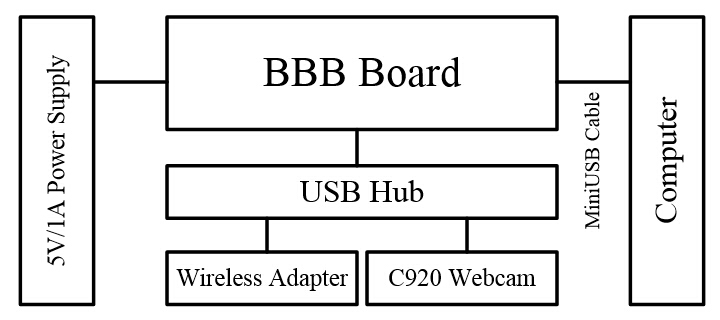
\includegraphics[width=4in]{./figs/hw1.jpg}
	\caption{Block diagram of hardware description.}
	\label{hw1}
\end{figure}
\begin{figure}[ht]
	\centering
	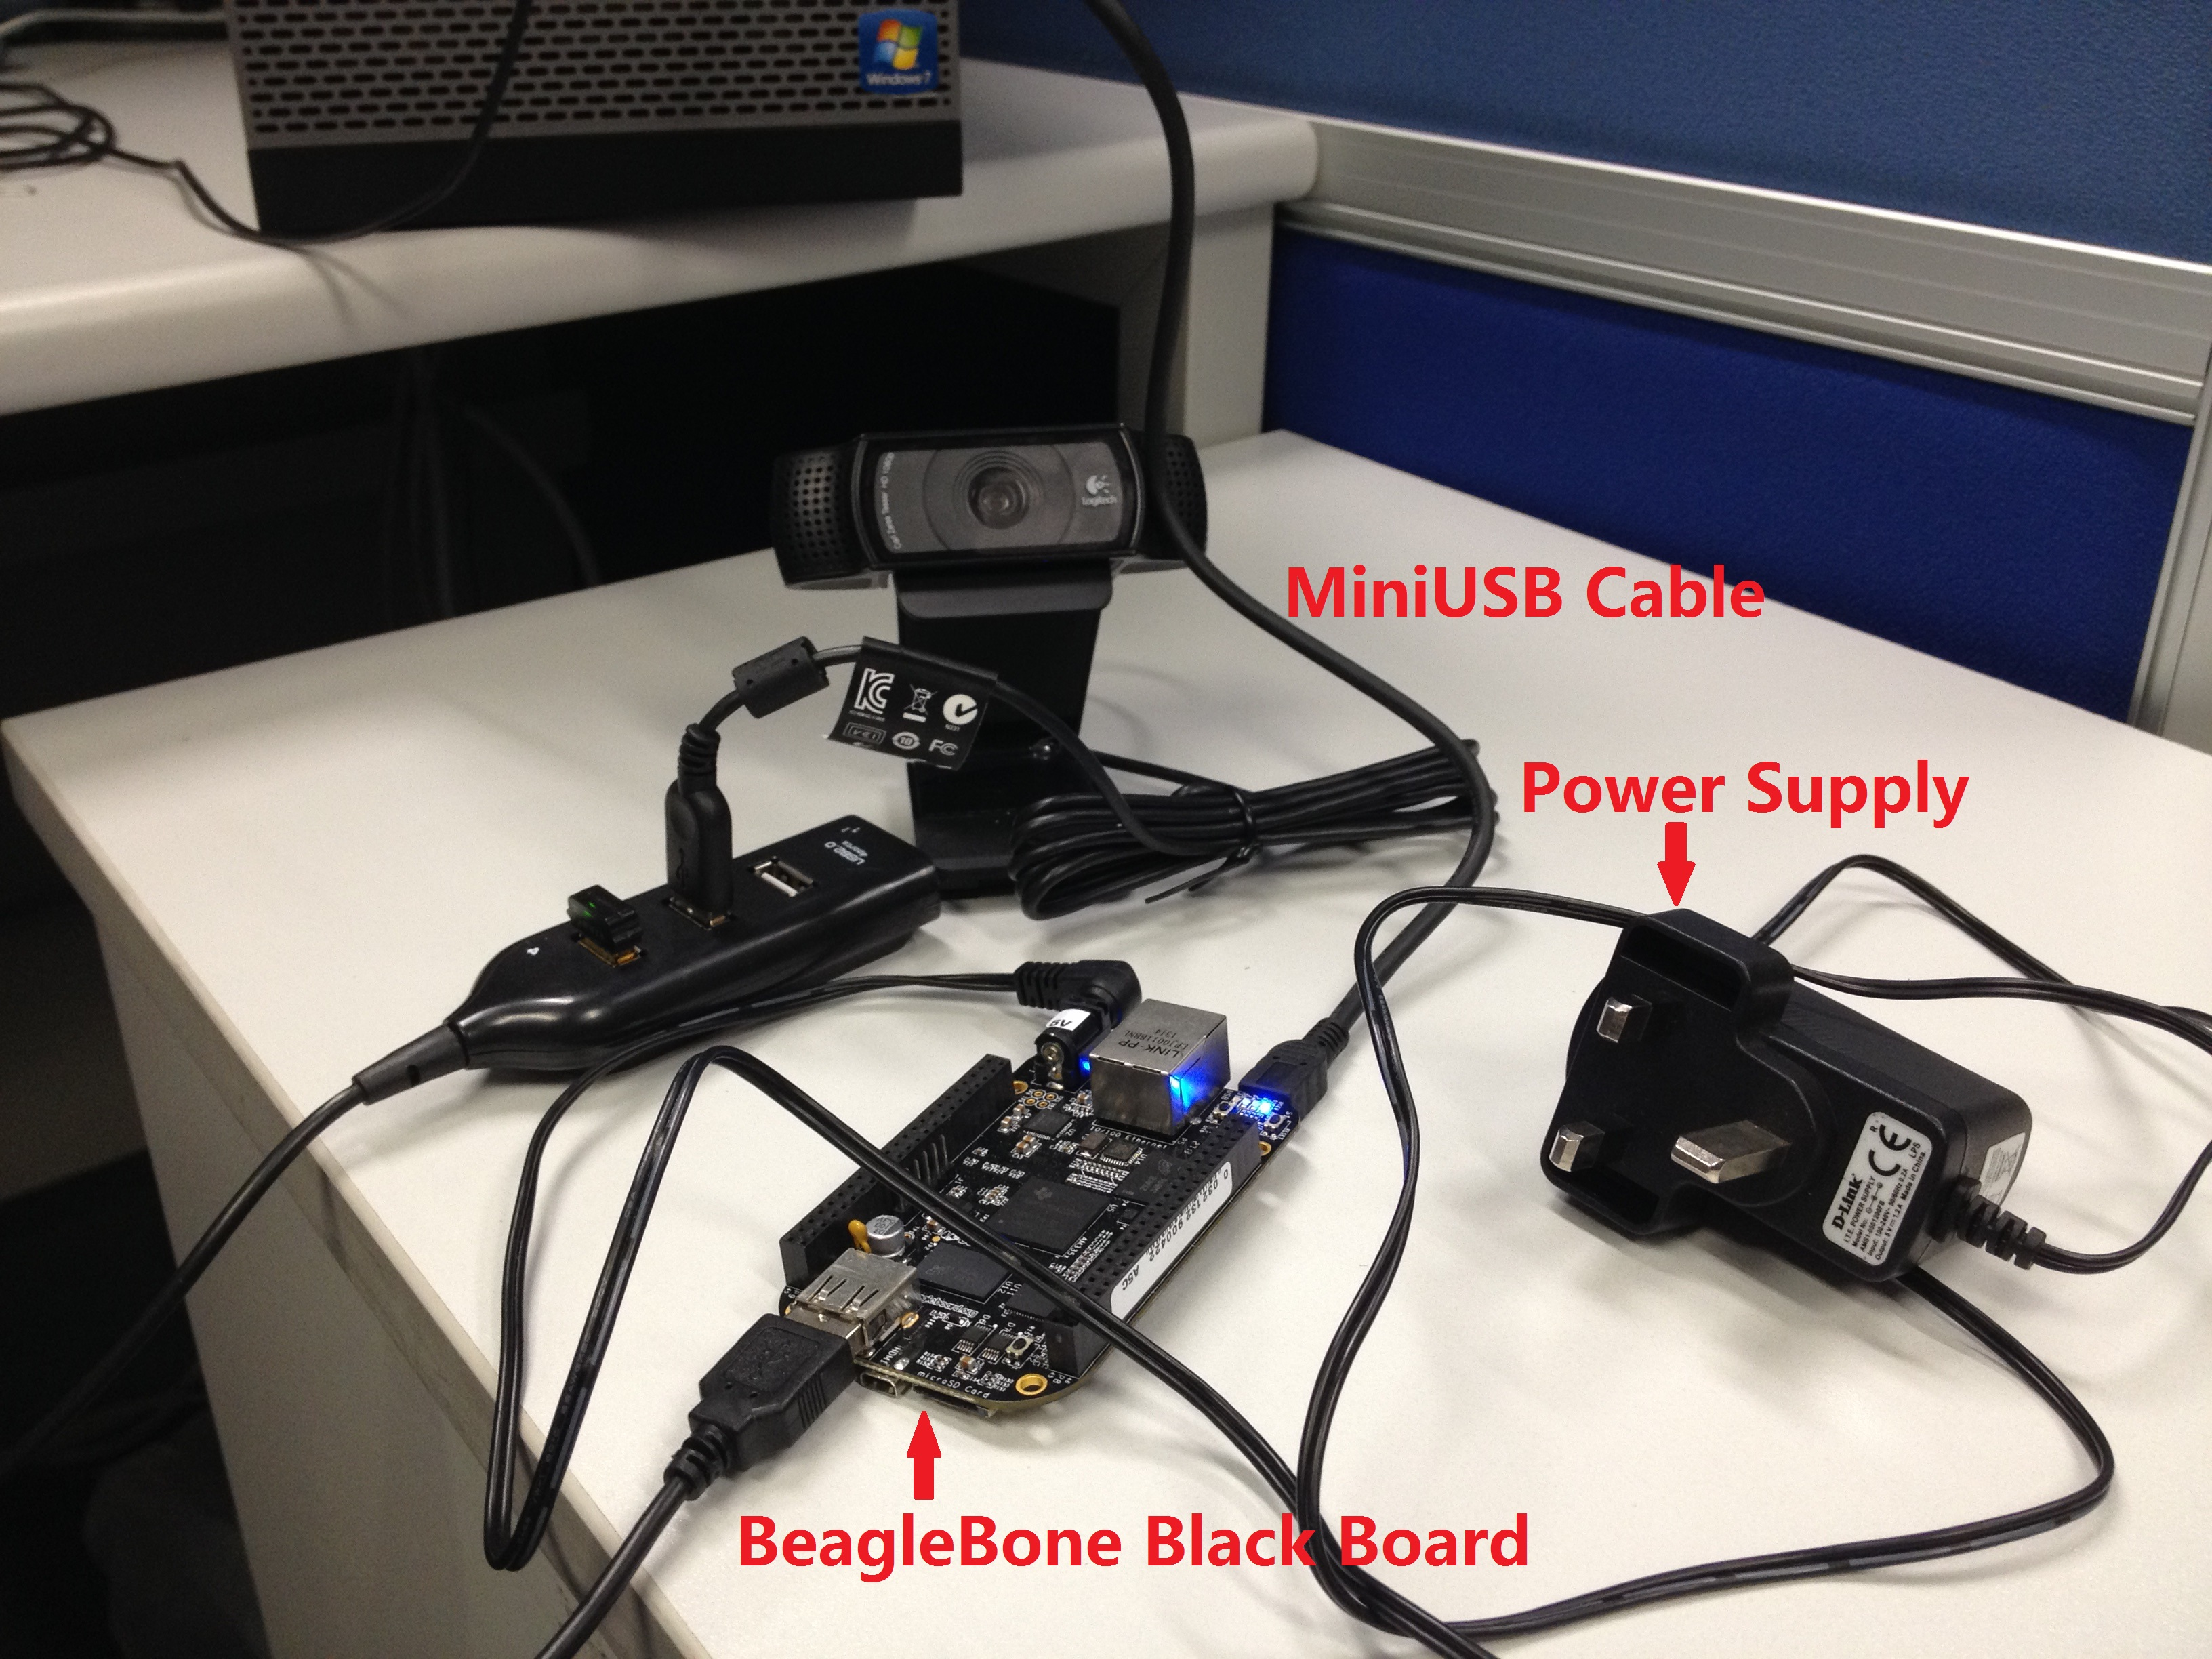
\includegraphics[width=4in]{./figs/hw2.jpg}
	\caption{Real view of hardware description.}
	\label{hw2}
\end{figure}

Both of the figures indicate the hardware setup details. First, the BBB board is connected to a PC using the MiniUSB Cable. Via the cable, the BBB board could not only receives a 5V/500mA power supply provided by PC's USB port, but also accesses to the Internet by setting up Windows ICS, in addition, users could operate Linux instructions through specific Windows-based software clients. Second, in case of unexpected system shutdown issue caused by current exceeding (current supply using MiniUSB Cable is set at a maximum of 500mA), an external power supply is used. Third, an USB Hub is connected to the onboard host USB port for expanding the port from one to four. Finally, the Logitech C920 webcam is connected to the USB Hub with its attached USB cable, together with a USB portable wireless adapter. Note that in this project, the BBB board could have an alternative way to access the Internet: getting access to a Wifi or a Hotspot connection via the wireless adapter; and the system could have two different IP address for Ethernet and wireless connection, respectively.


% % % % % % % % % % % % % % % % % % % % % % % % % % % % % % % % %
% % % % % % % % % % % % % % % % % % % % % % % % % % % % % % % % %
\section{Software Description and Implementation}\label{SfDes}
	
	\subsection{Operating System Installation and Configuration}\label{Sys}
	In our implementation, we install Ubuntu Trusty 14.04 on BBB. This image uses the Ubuntu 14.04 core filesystem from Ubuntu with the minimal meta package applied. The kernel is compiled from the mainline Linux kernel git repository. The result is an easy-to-install and stable Linux image that works well with the BeagleBone Black boards.

First, OS binaries ``ubuntu-trusty-14.04-rootfs-3.14.4.1-bone-armhf.com.tar.xz" should be downloaded from \textit{\url{http://www.armhf.com/boards/beaglebone-black/}}; After uncompressing this file, we can get the Ubuntu Trusty 14.04 image as shown in Fig. \ref{osimage}. Next, this image should be burn into a microSD card such that we can install Ubuntu 14.04 onto BeagleBone Black. One way of doing this task is by utilizing Win32DiskImager, which is a powerful tool automatically creating a OS boot disk and available at \textit{\url{http://sourceforge.net/projects/win32diskimager/files/latest/download}}. In Fig. , Win32DiskImager starts to write Ubuntu .img to the microSD card, as presented by `device' F:.

\begin{figure}[htb]
	\centering
	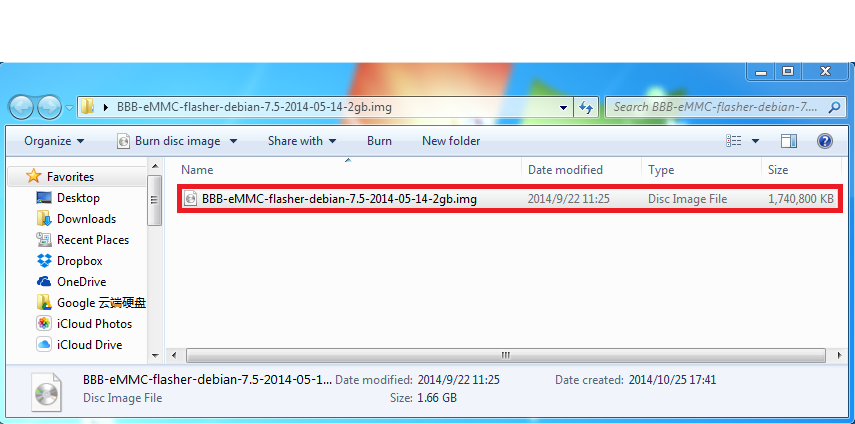
\includegraphics[width=5in]{./figs/osimage.PNG}
	\caption{Ubuntu Trusty 14.04 Image.}
	\label{osimage}
\end{figure}

\begin{figure}[htb]
	\centering
    \subfigure[MicroSD card.]{
       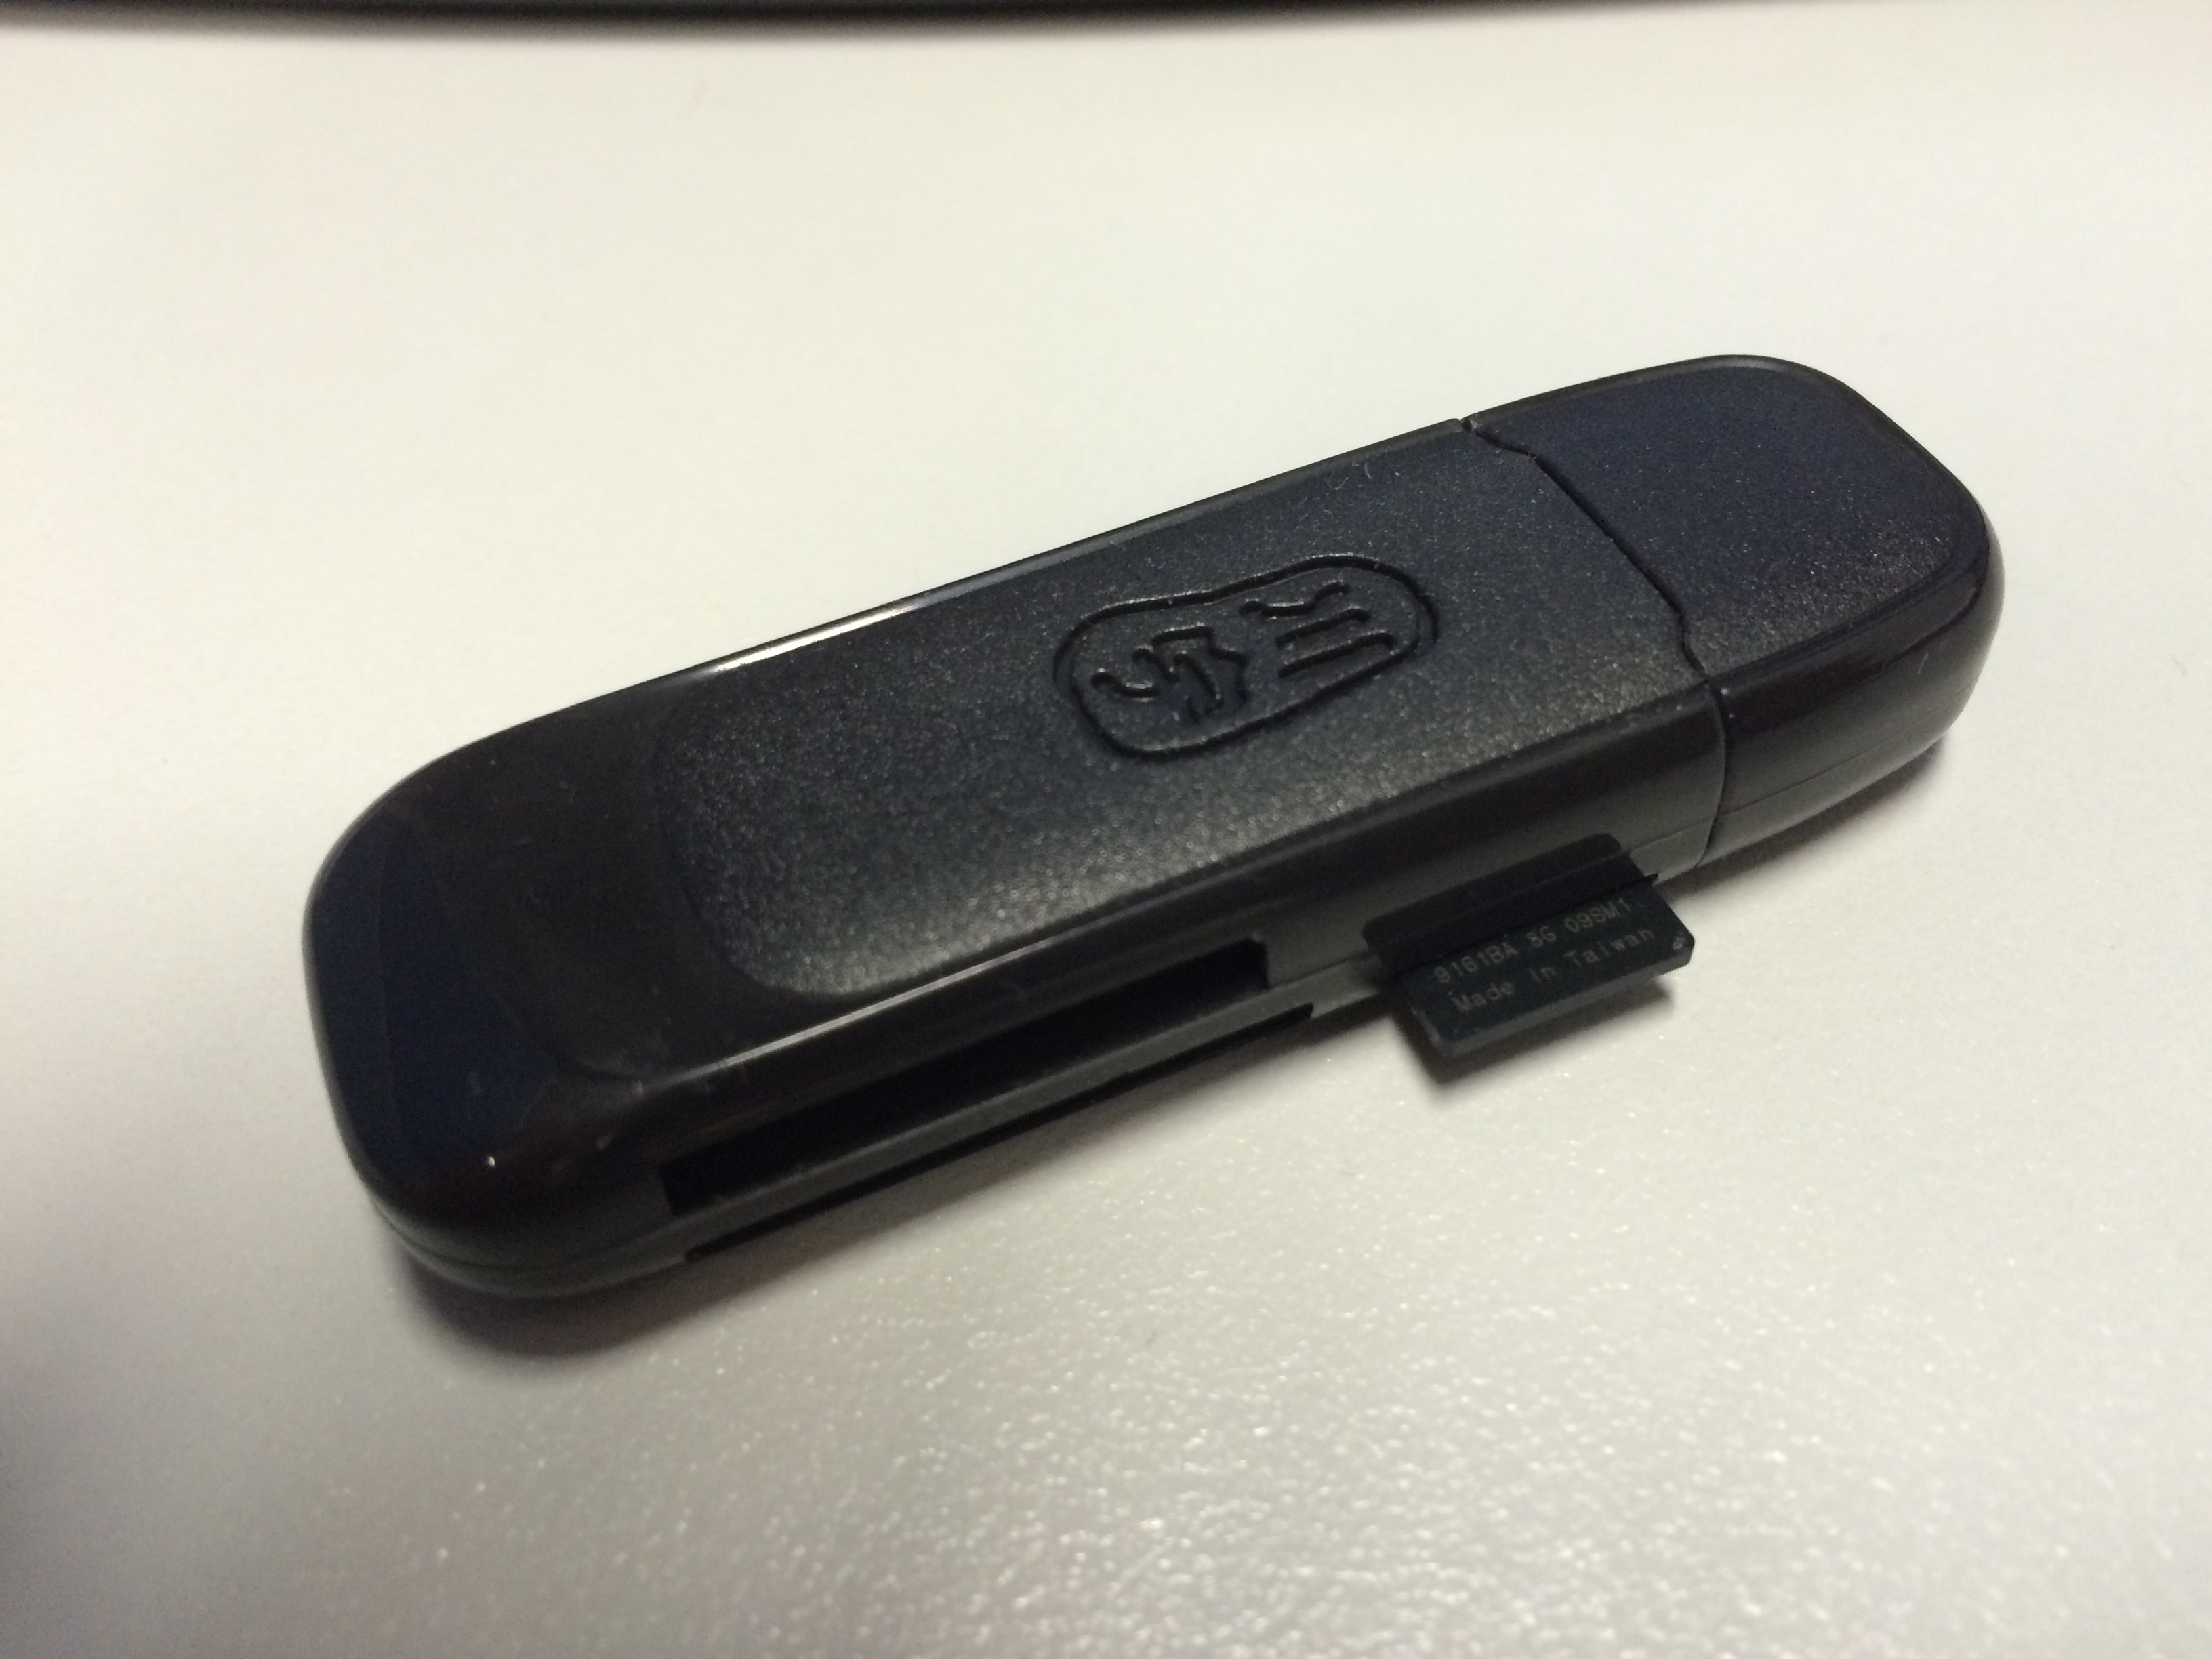
\includegraphics[width=2in]{./figs/microsd.JPG}
       \label{microsd}
     }
    \subfigure[Win32DiskImager]{
       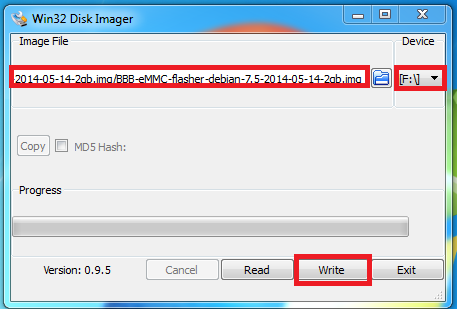
\includegraphics[width=3in]{./figs/win32diskimager.PNG}
       \label{win32diskimager}
     }
     \caption{Creating A Ubuntu bootable image on microSD card.}
     \end{figure}
     
When the microSD Card is now ready to boot, we insert it into BeagleBone Black board, hold down the USER/BOOT button (in our board, it is S3 button.) and apply power, either by the USB cable or 5V adapter. However, it is strongly recommended to plug the 5V adapter in all the time because power adapter can provide more stable voltage than USB cable and thus it is less likely to have unexpected problems caused by power cutoff or insufficient. 

Keep holding down the button until  the bank of 4 LED's light up for a few seconds and now release the button.
It will take anywhere from 30-45 minutes to flash the image onto the on-board chip. Once it's done, the bank of 4 LED's to the right of the Ethernet will all stay lit up at the same time. We can then power down your BeagleBone Black[]. One important thing worth mentioning is that after finishing this step, we do not need microSD card installation anymore --- you can plug it out and whenever you power the board again, Ubuntu is able to automatically boot from MMC, the inner storage component on chip.
	
\subsection{Wireless Adapter Configuration}\label{Wireless}
Once the OS is successfully set up on board, it becomes critical to have internet access --- We need to install extra system utilities or download third-party libraries to support this project. So in this section, we detail how to setup a WiFi connection for BeagleBone Black.

To begin with, we must connect the components needed into BeagleBone: wireless network adapter, USB hub and miniUSB cable (See Fig.). The wireless network adapter is the key for Internet connectivity. Besides this adapter, a webcam is also required by this project but we only have one USB port for them.  We therefore use a USB hub to install both components. We also need a miniUSB cable to connect BeagleBone to the host PC such that we can remote control BeagleBone through host PC's keyboard. Or to be more precise, we start a SSH connection to BeagleBone through this cable.
  
\begin{figure}[htb]
	\centering
    \subfigure[Wireless Network Adapter]{
       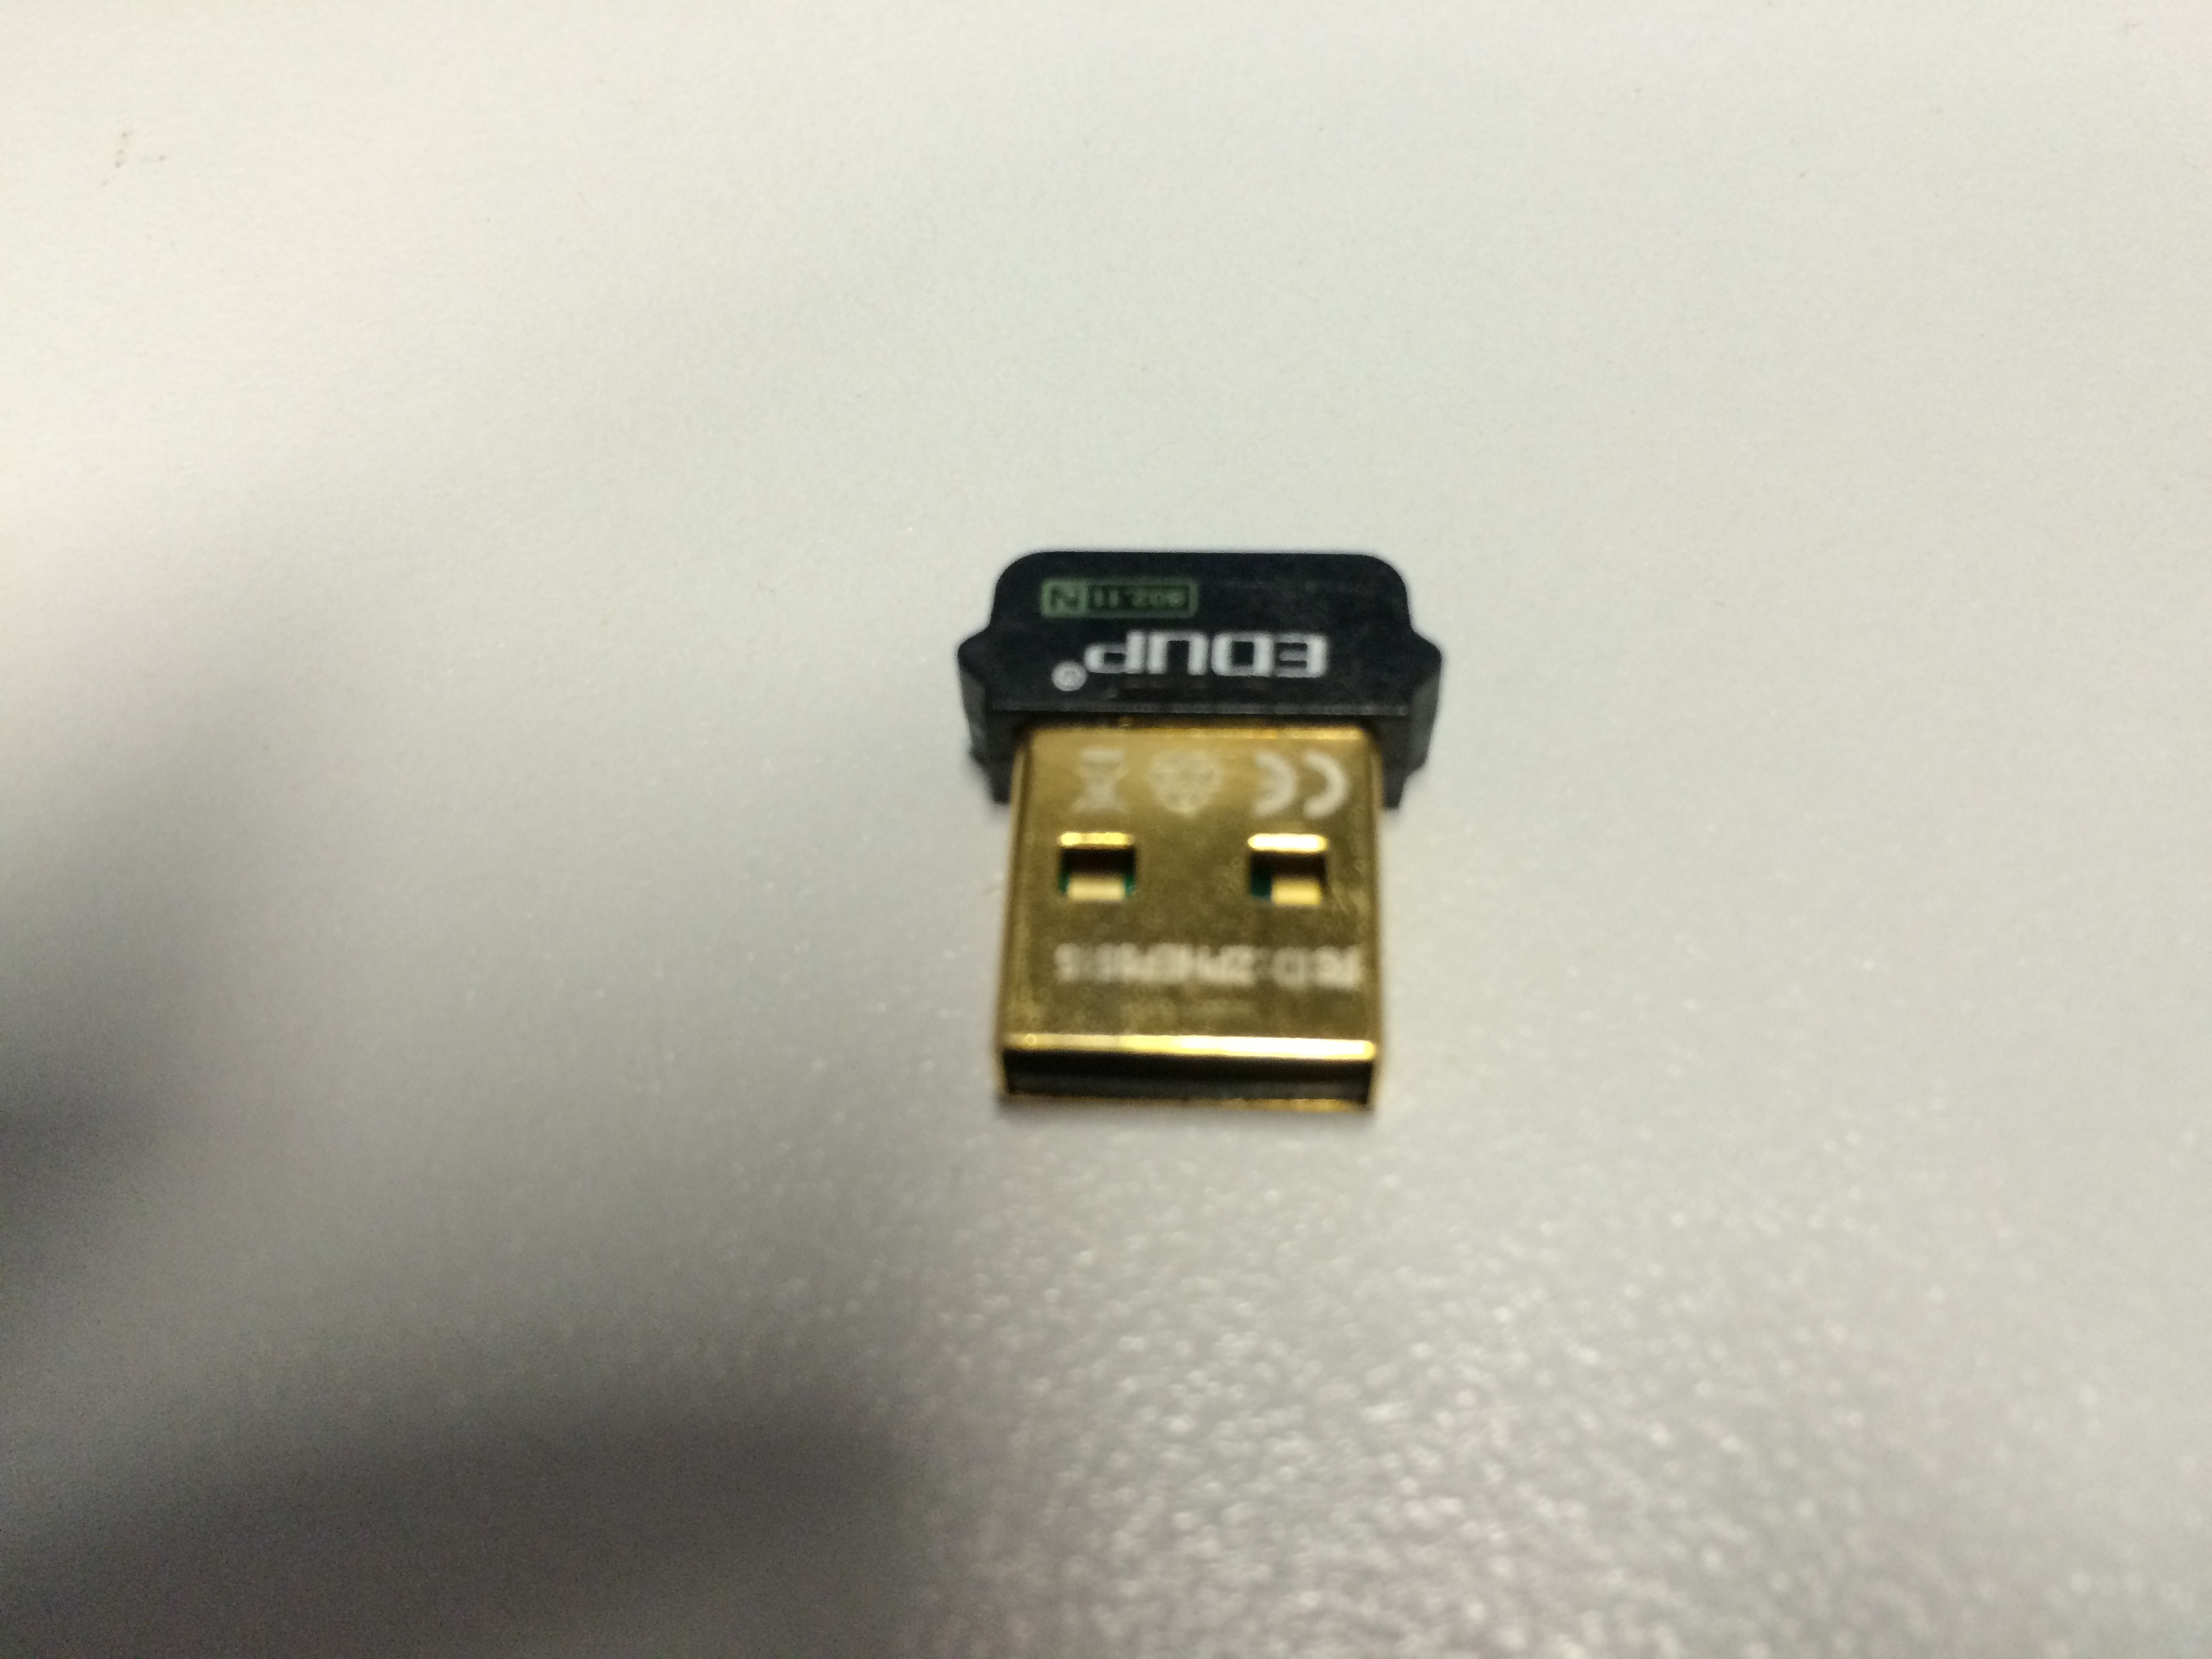
\includegraphics[width=2in]{./figs/wifiadapter.JPG}
       \label{wirelessadapter.PNG}
     }
    \subfigure[Usb Hub]{
       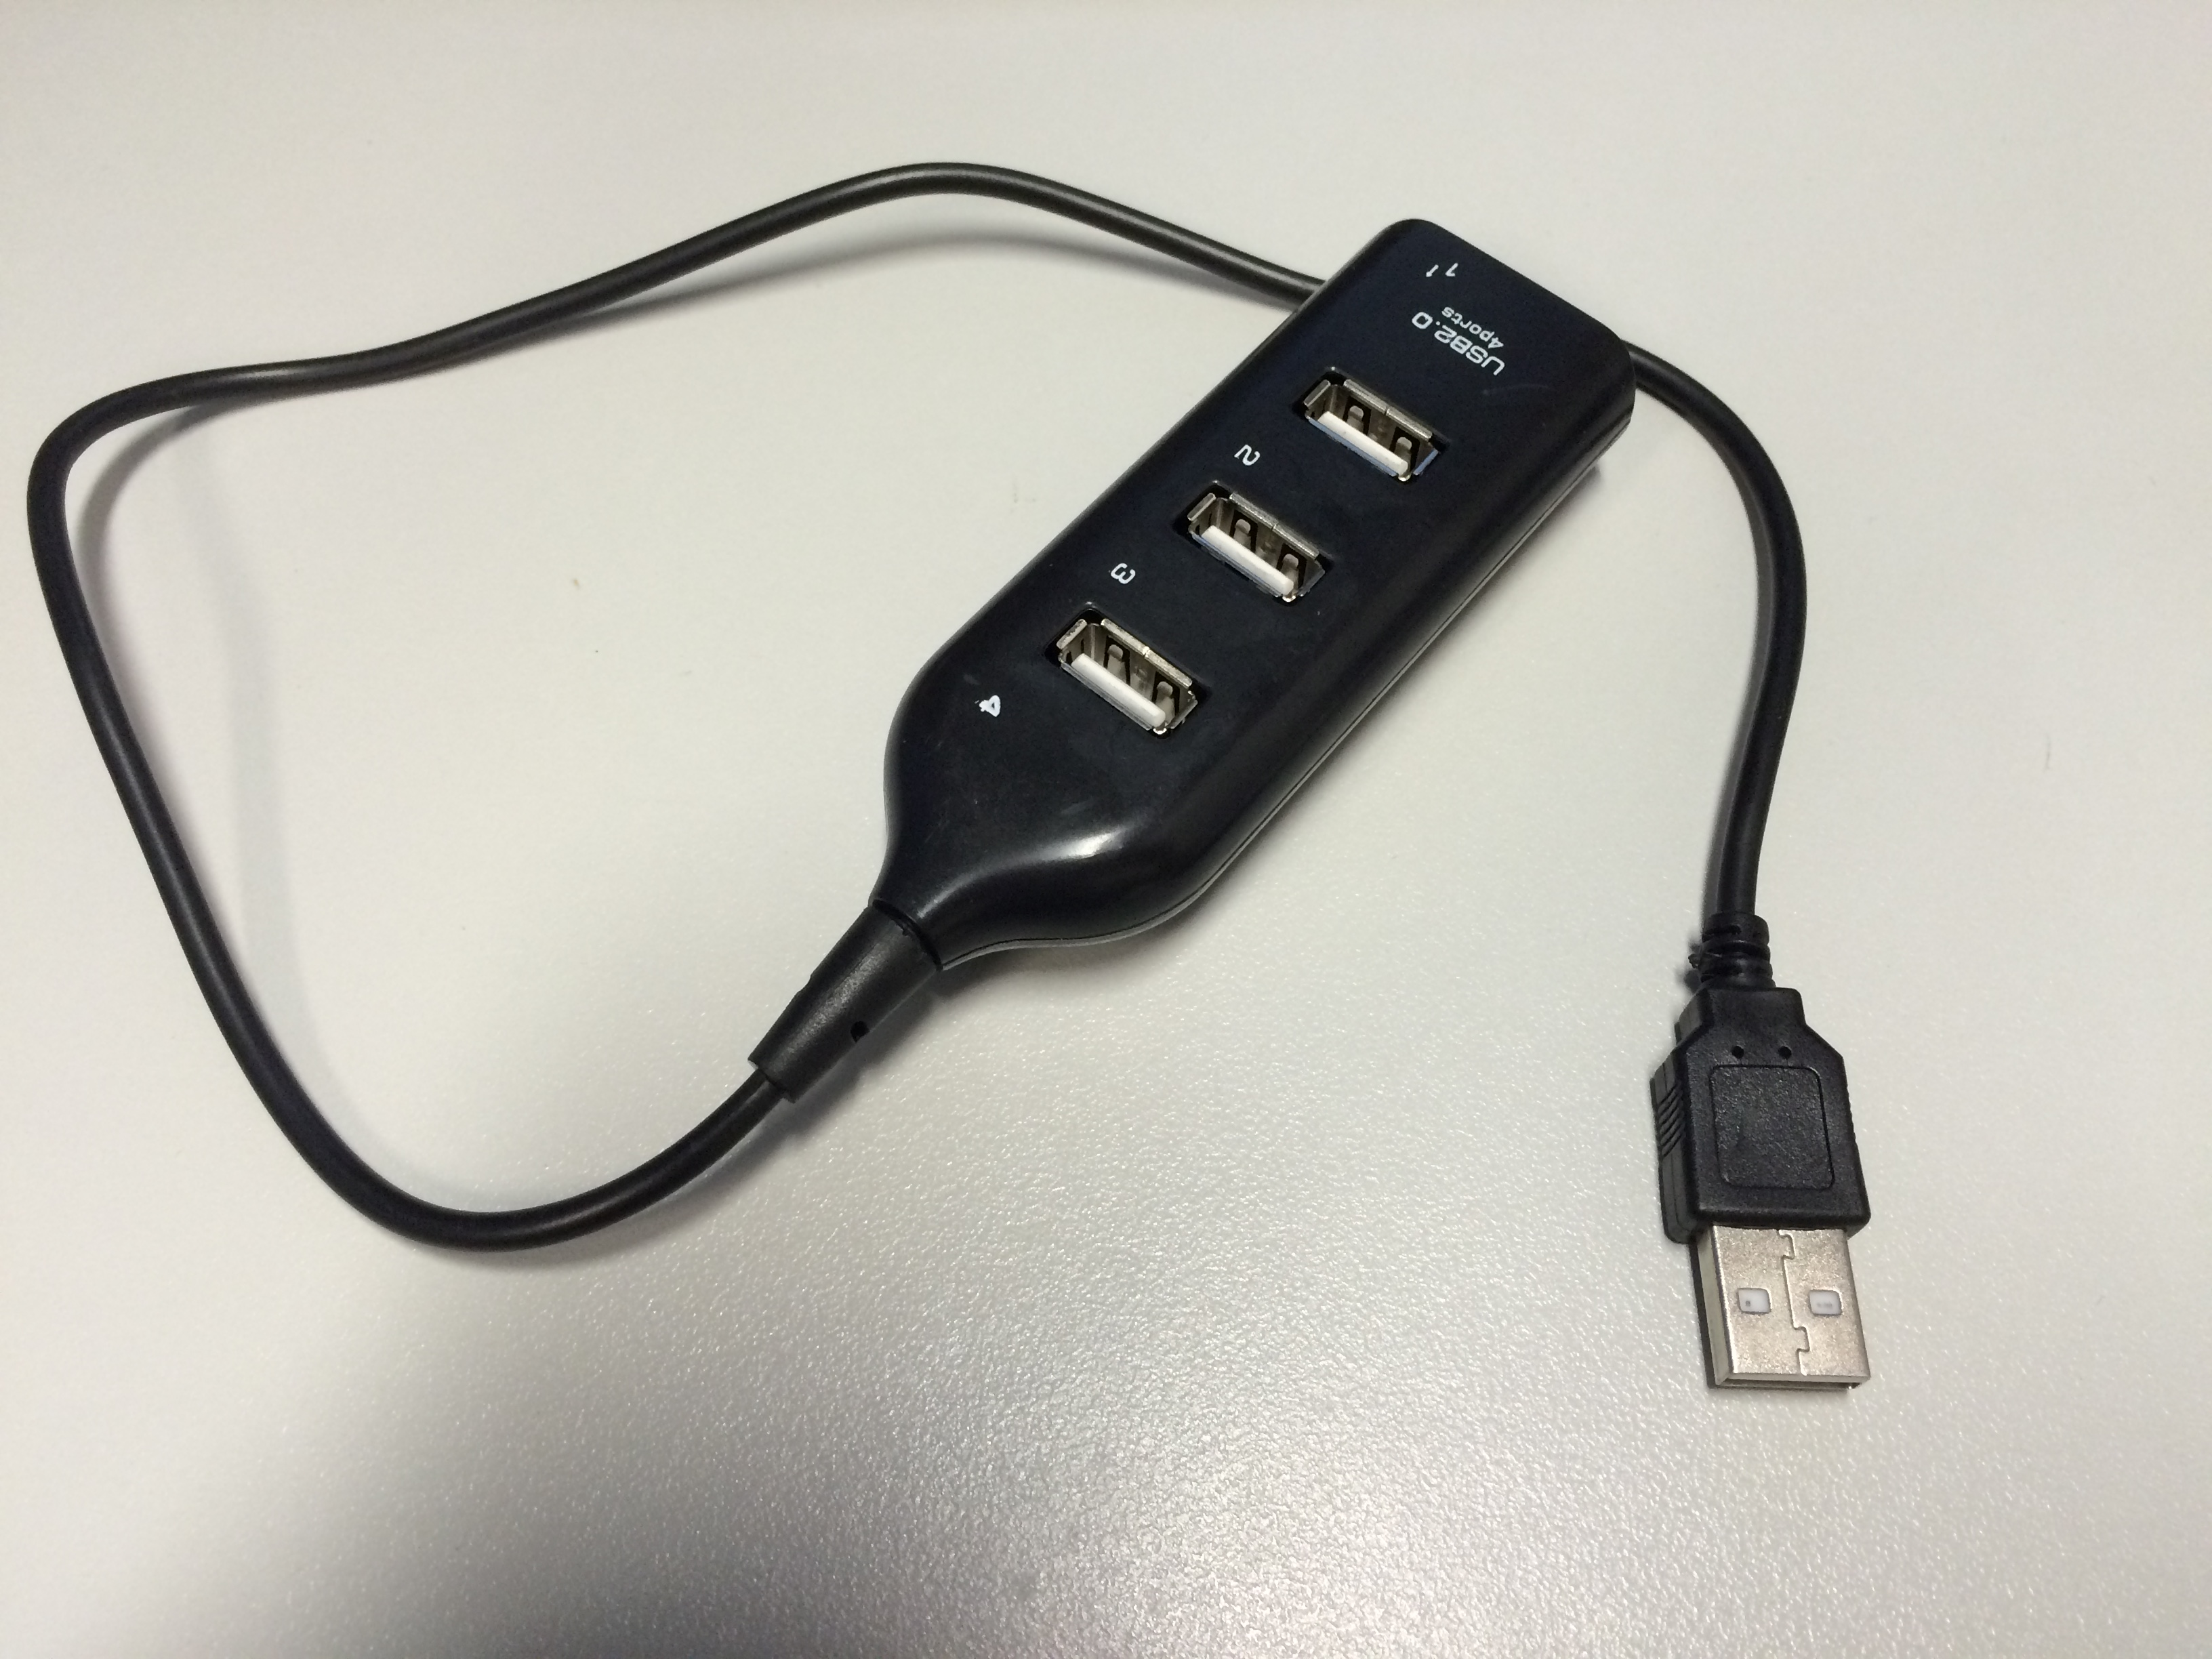
\includegraphics[width=2in]{./figs/usbhub.JPG}
       \label{usbhub.PNG}
     }
     \subfigure[MiniUSB cable]{
       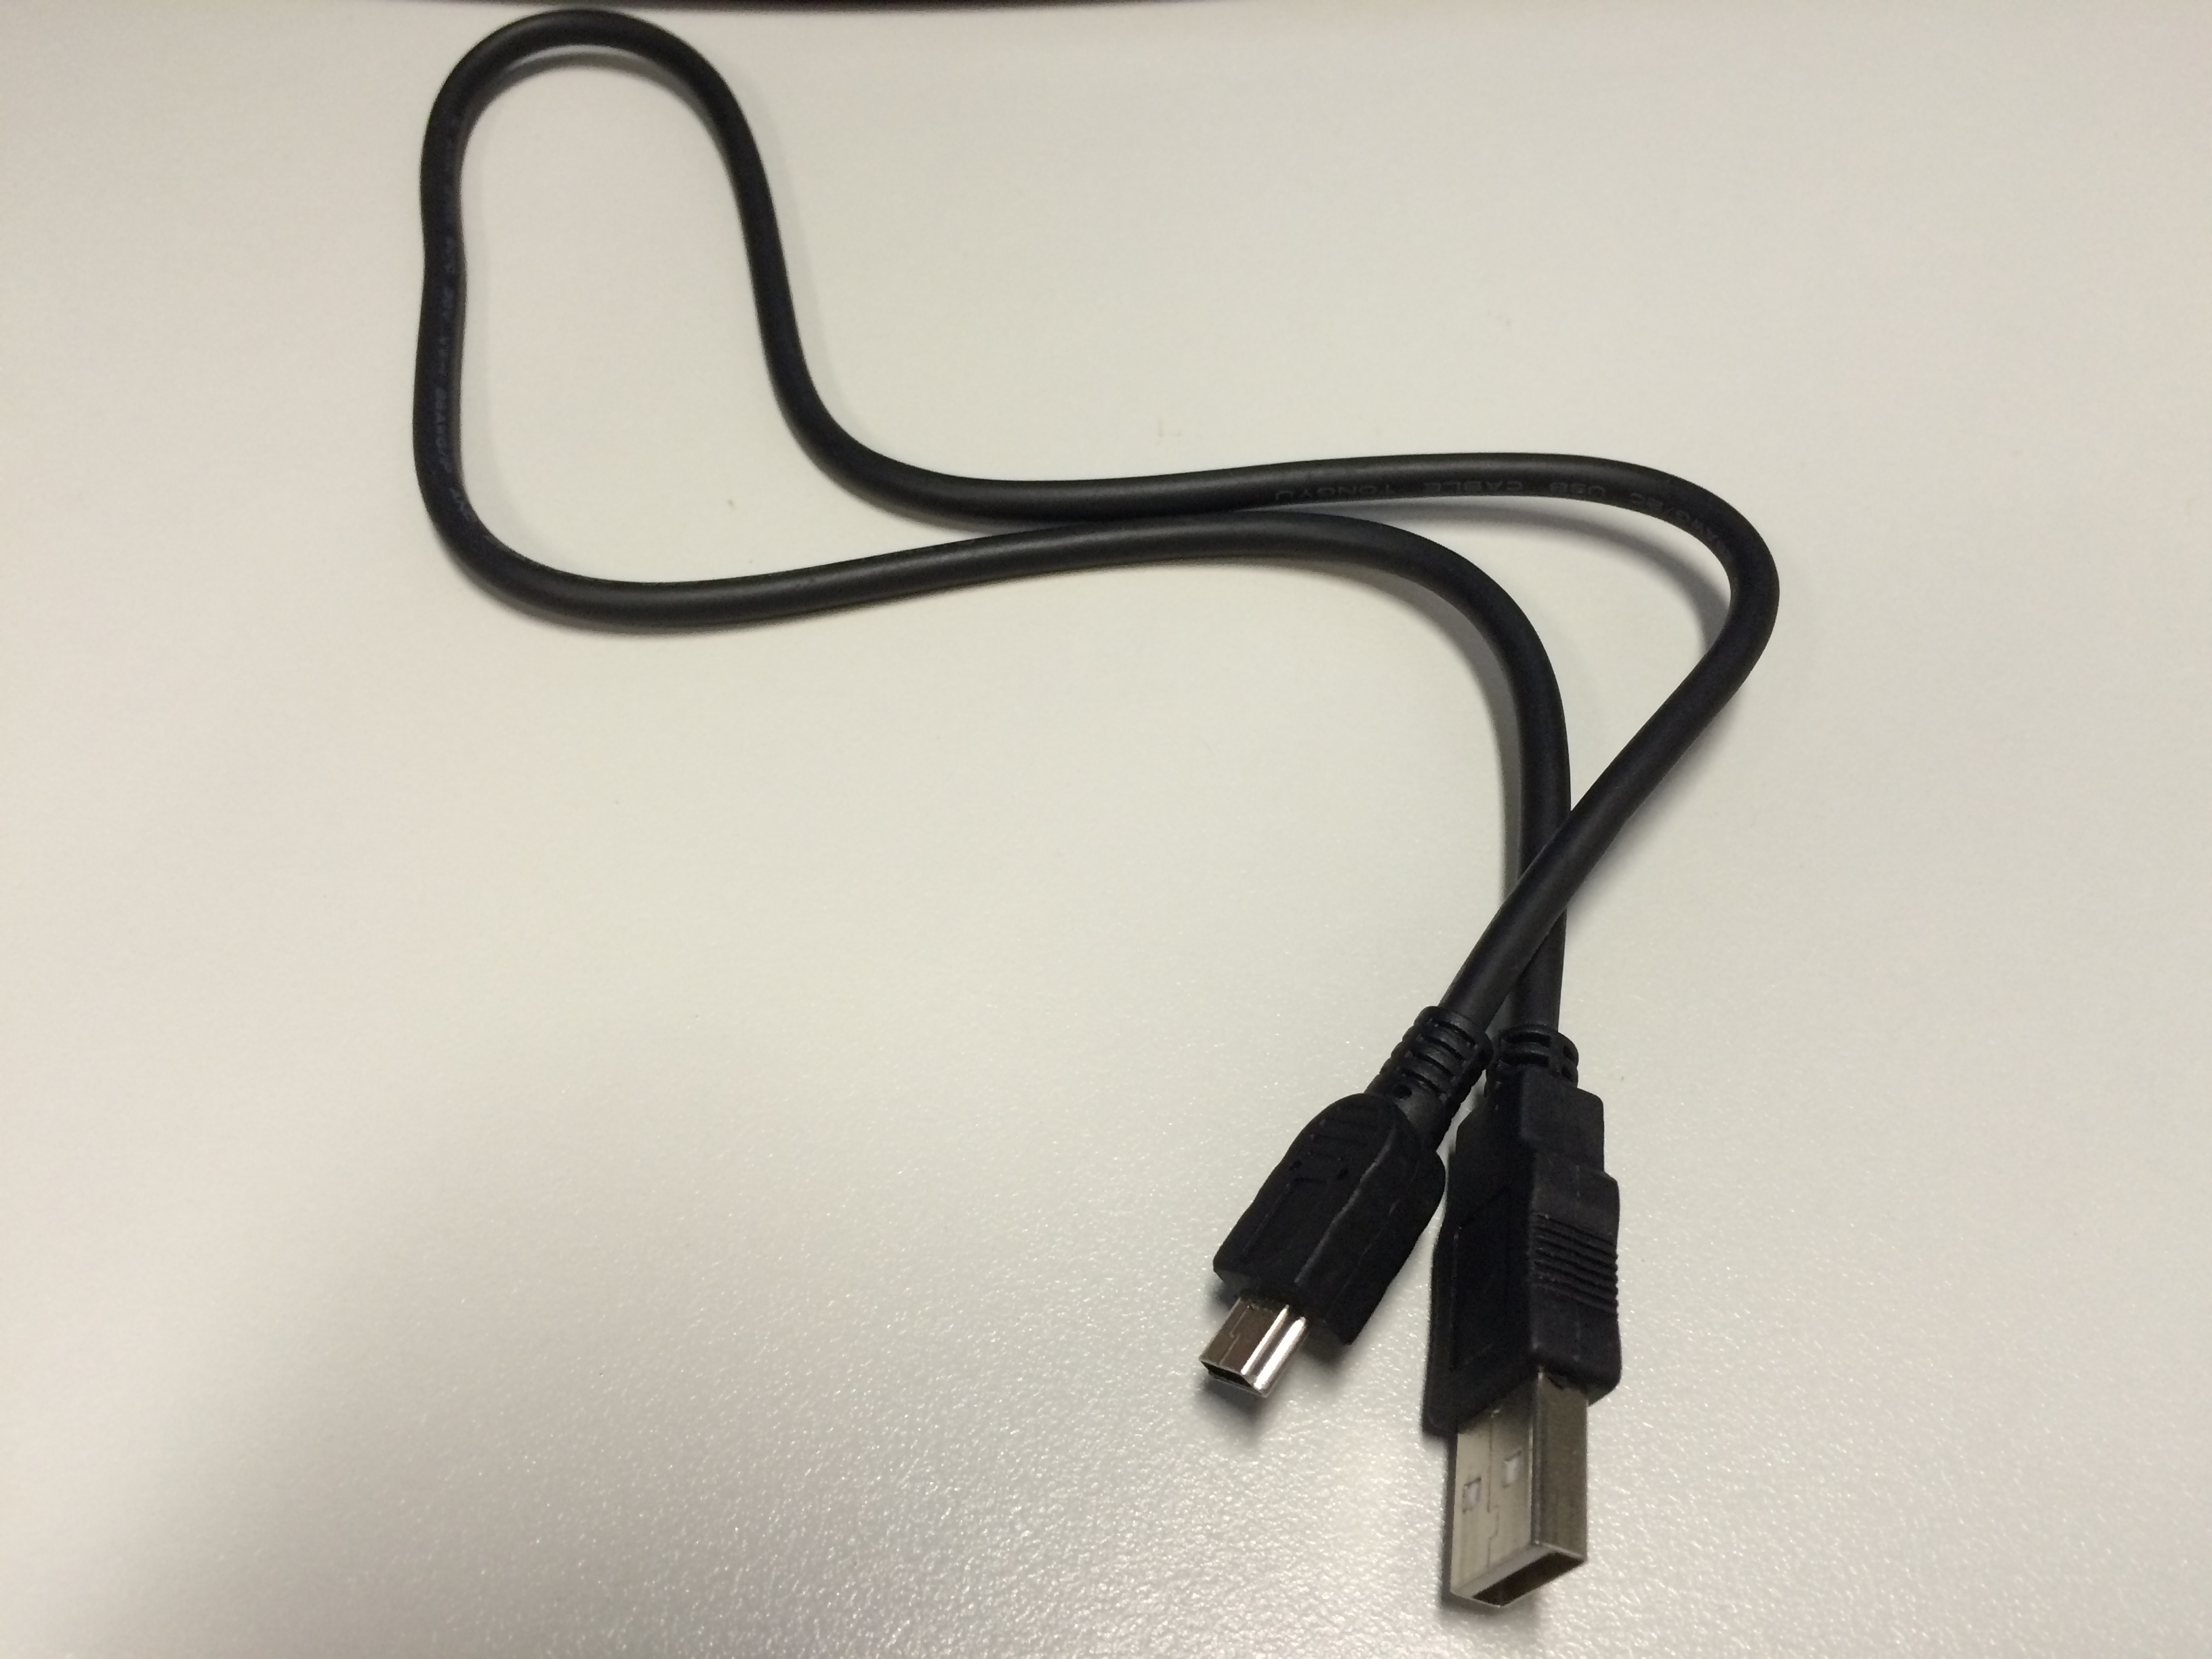
\includegraphics[width=2in]{./figs/miniusbcable.JPG}
       \label{usbhub.PNG}
     }
     \caption{Essential components for WiFi connection}
     \end{figure}  
  
To establish SSH connection, we must log on BeagleBone via SSH protocol and this could be done with the help of SSH tool. In fact, there are a variety of SSH GUI tools available for Windows. In this report, we take Secure Shell Client available on \textit{\url{http://mepopedia.com/forum/file.php?793,file=1103,filename=SSHSecureShellClient-3.2.9.exe,download=1}}  as an example because this tool integrates scp command that allows us to transfer files between the host PC and the BeagleBone freely.

When the wireless network adapter is plug into BeagleBone and BeagleBone itself is also connected to one USB port on our host PC, we open the Secure Shell Client and start a SSH connection from PC to BeagleBone as shown in Fig. \ref{ssh}. Remember the default IP address for BeagleBone is 192.168.7.2 and the default user account is `ubuntu' with password "temppwd".
\begin{figure}[htb]
	\centering

    \subfigure{
       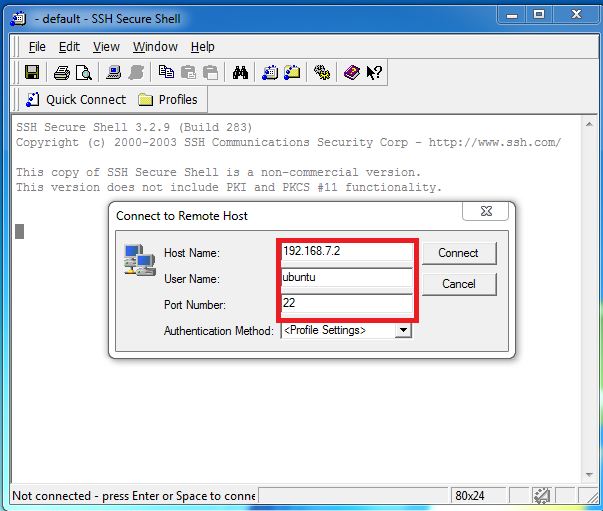
\includegraphics[width=3in]{./figs/ssh1.PNG}

     }
    \subfigure{
       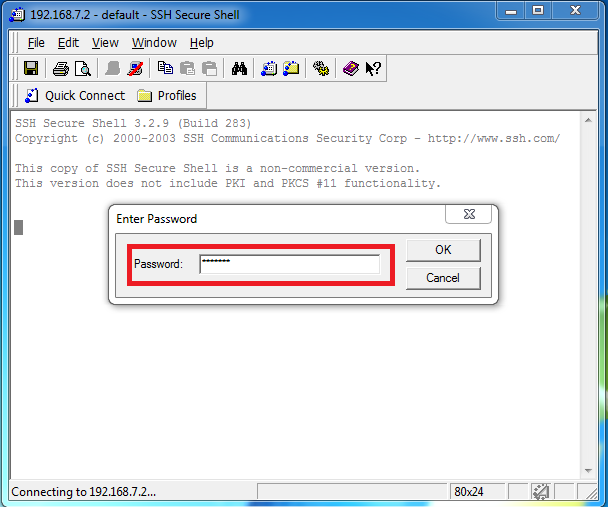
\includegraphics[width=3in]{./figs/ssh2.PNG}

     }
     \caption{SSH log on via Secure Shell Client for Windows.}\label{ssh}
     \end{figure}
     
Finally, we configure the WiFi setup by modifying the network configuration file located at /ect/network/interfaces. 
In figure \ref{wifi} we present the changes that have been made marked in red box. The idea of the is to connect to CityU Campus Wifi network --- "Universities WiFi" with the student EID and password. For safety reason, the EID and password are wiped out and readers can use their own account to fill in.

\begin{figure}[htb]
	\centering
	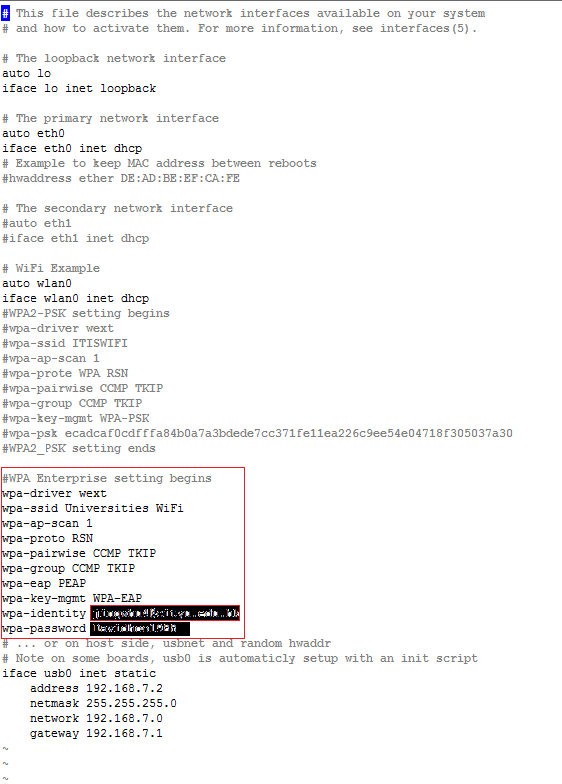
\includegraphics[width=5in]{./figs/wifi.PNG}
	\caption{Modify /ect/network/interfaces to establish a WiFi connection to access the Internet.}
	\label{wifi}
\end{figure}

To make the modifications into effect, we type in "ifconfig wlan0 down $\&\&$ ifconfig wlan0 up" from Secure Shell Client to restart the wirless adapter. Then we type in "ping www.google.com.hk" to test whether the WiFi connection is functioning. Fig. \ref{ping} shows that the network setup is correct with all 4 transmitted packets getting received.

\begin{figure}[htb]
	\centering
	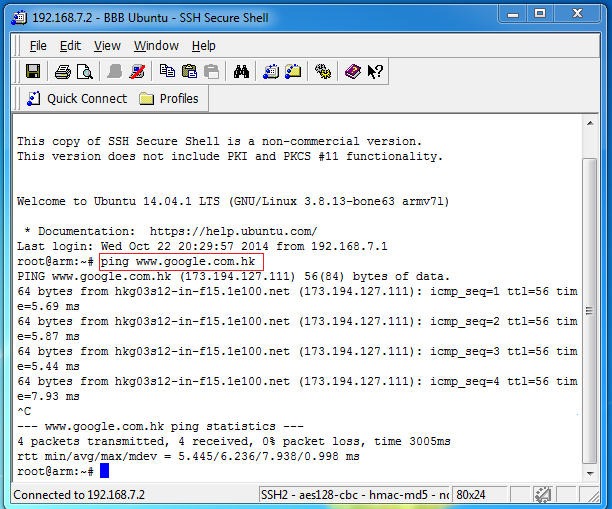
\includegraphics[width=4in]{./figs/ping.PNG}
	\caption{A successful ping to Google.}
	\label{ping}
\end{figure}

One last reminder is that we suggest to log in as `root' rather than `ubuntu'. This is primarily because `ubuntu' does have full access to all system resources and in many cases, you would get errors like `permission denied'. Just switch to `root' and all these annoying errors disappear.

\subsection{Web Server Setup}\label{Webser}
	
\subsection{LED Test}\label{Led}
	
\subsection{Web Camera Configuration and Functioning}\label{Webcam}

\subsection{SQL Server Setup and Application}\label{Sql}
	
\section{Conclusions}\label{Con}

% % % % % % % % % % % % % % % % % % % % % % % % % % % % % % % % %
% % % % % % % % % % % % % % % % % % % % % % % % % % % % % % % % %
\section*{Acknowledgment}
We would like to thank our colleague Sean Yang  for his kindly help with the WiFi setup on BBB board.


%\begin{thebibliography}{1}
%\item
%\end{thebibliography}
%\bibliographystyle{latex8} \bibliography{latex8}

\end{document}



%\bibliographystyle{plain}
%\bibliography{source}

